\documentclass{article}

% Language setting
% Replace `english' with e.g. `spanish' to change the document language
\usepackage[english]{babel}

% Set page size and margins
% Replace `letterpaper' with `a4paper' for UK/EU standard size
\usepackage[letterpaper,top=2cm,bottom=2cm,left=3cm,right=3cm,marginparwidth=1.75cm]{geometry}

% Useful packages
\usepackage{amsmath}
\usepackage{graphicx}
\usepackage[colorlinks=true, allcolors=blue]{hyperref}

\title{PS6 Smith}

\begin{document}
\maketitle

\section{Question 3 Data Cleaning}
I used my FRED API key to pull the \textbf{\href{https://fred.stlouisfed.org/series/PCU3334133341}{data}} of the HVAC and Commercial Refrigeration Equipment Producer Price Index.

To clean up the data, I performed the following steps:
\begin{enumerate}
    \item Named the data file and saved as a data frame
    \item converted the Date column to a date format
    \item Renamed the column providing the date the data was pulled and removed the 'end-date' of data pulled since it was redundant
    \item filtered the data to only look at the last 5 years
    \item Added a percentage change column, calculated from value with respect to the older date
    \item Created a secondary data frame for my last chart to show the data by year and quarter. I also added a column for the percentage change quarter to quarter
\end{enumerate}


\space

\section{Question 4 Plot A}

\begin{enumerate}
    \item The first Time series, Figure 1, plot displays the HVAC Producer Price Index over the last 5 years. I like this chart because it shows the rapid rate of increase in pricing over the last five years. It also shows that while there have been some small dips in 2023, the value continues to climb. This is one way for me to combat discussions from our sales people when they say we should be getting price decreases because commodity prices have gone down. With more time, it would be good to find a way to layer in the commodity pricing of steel, copper and also labor rates.
    \begin{figure}
        \centering
        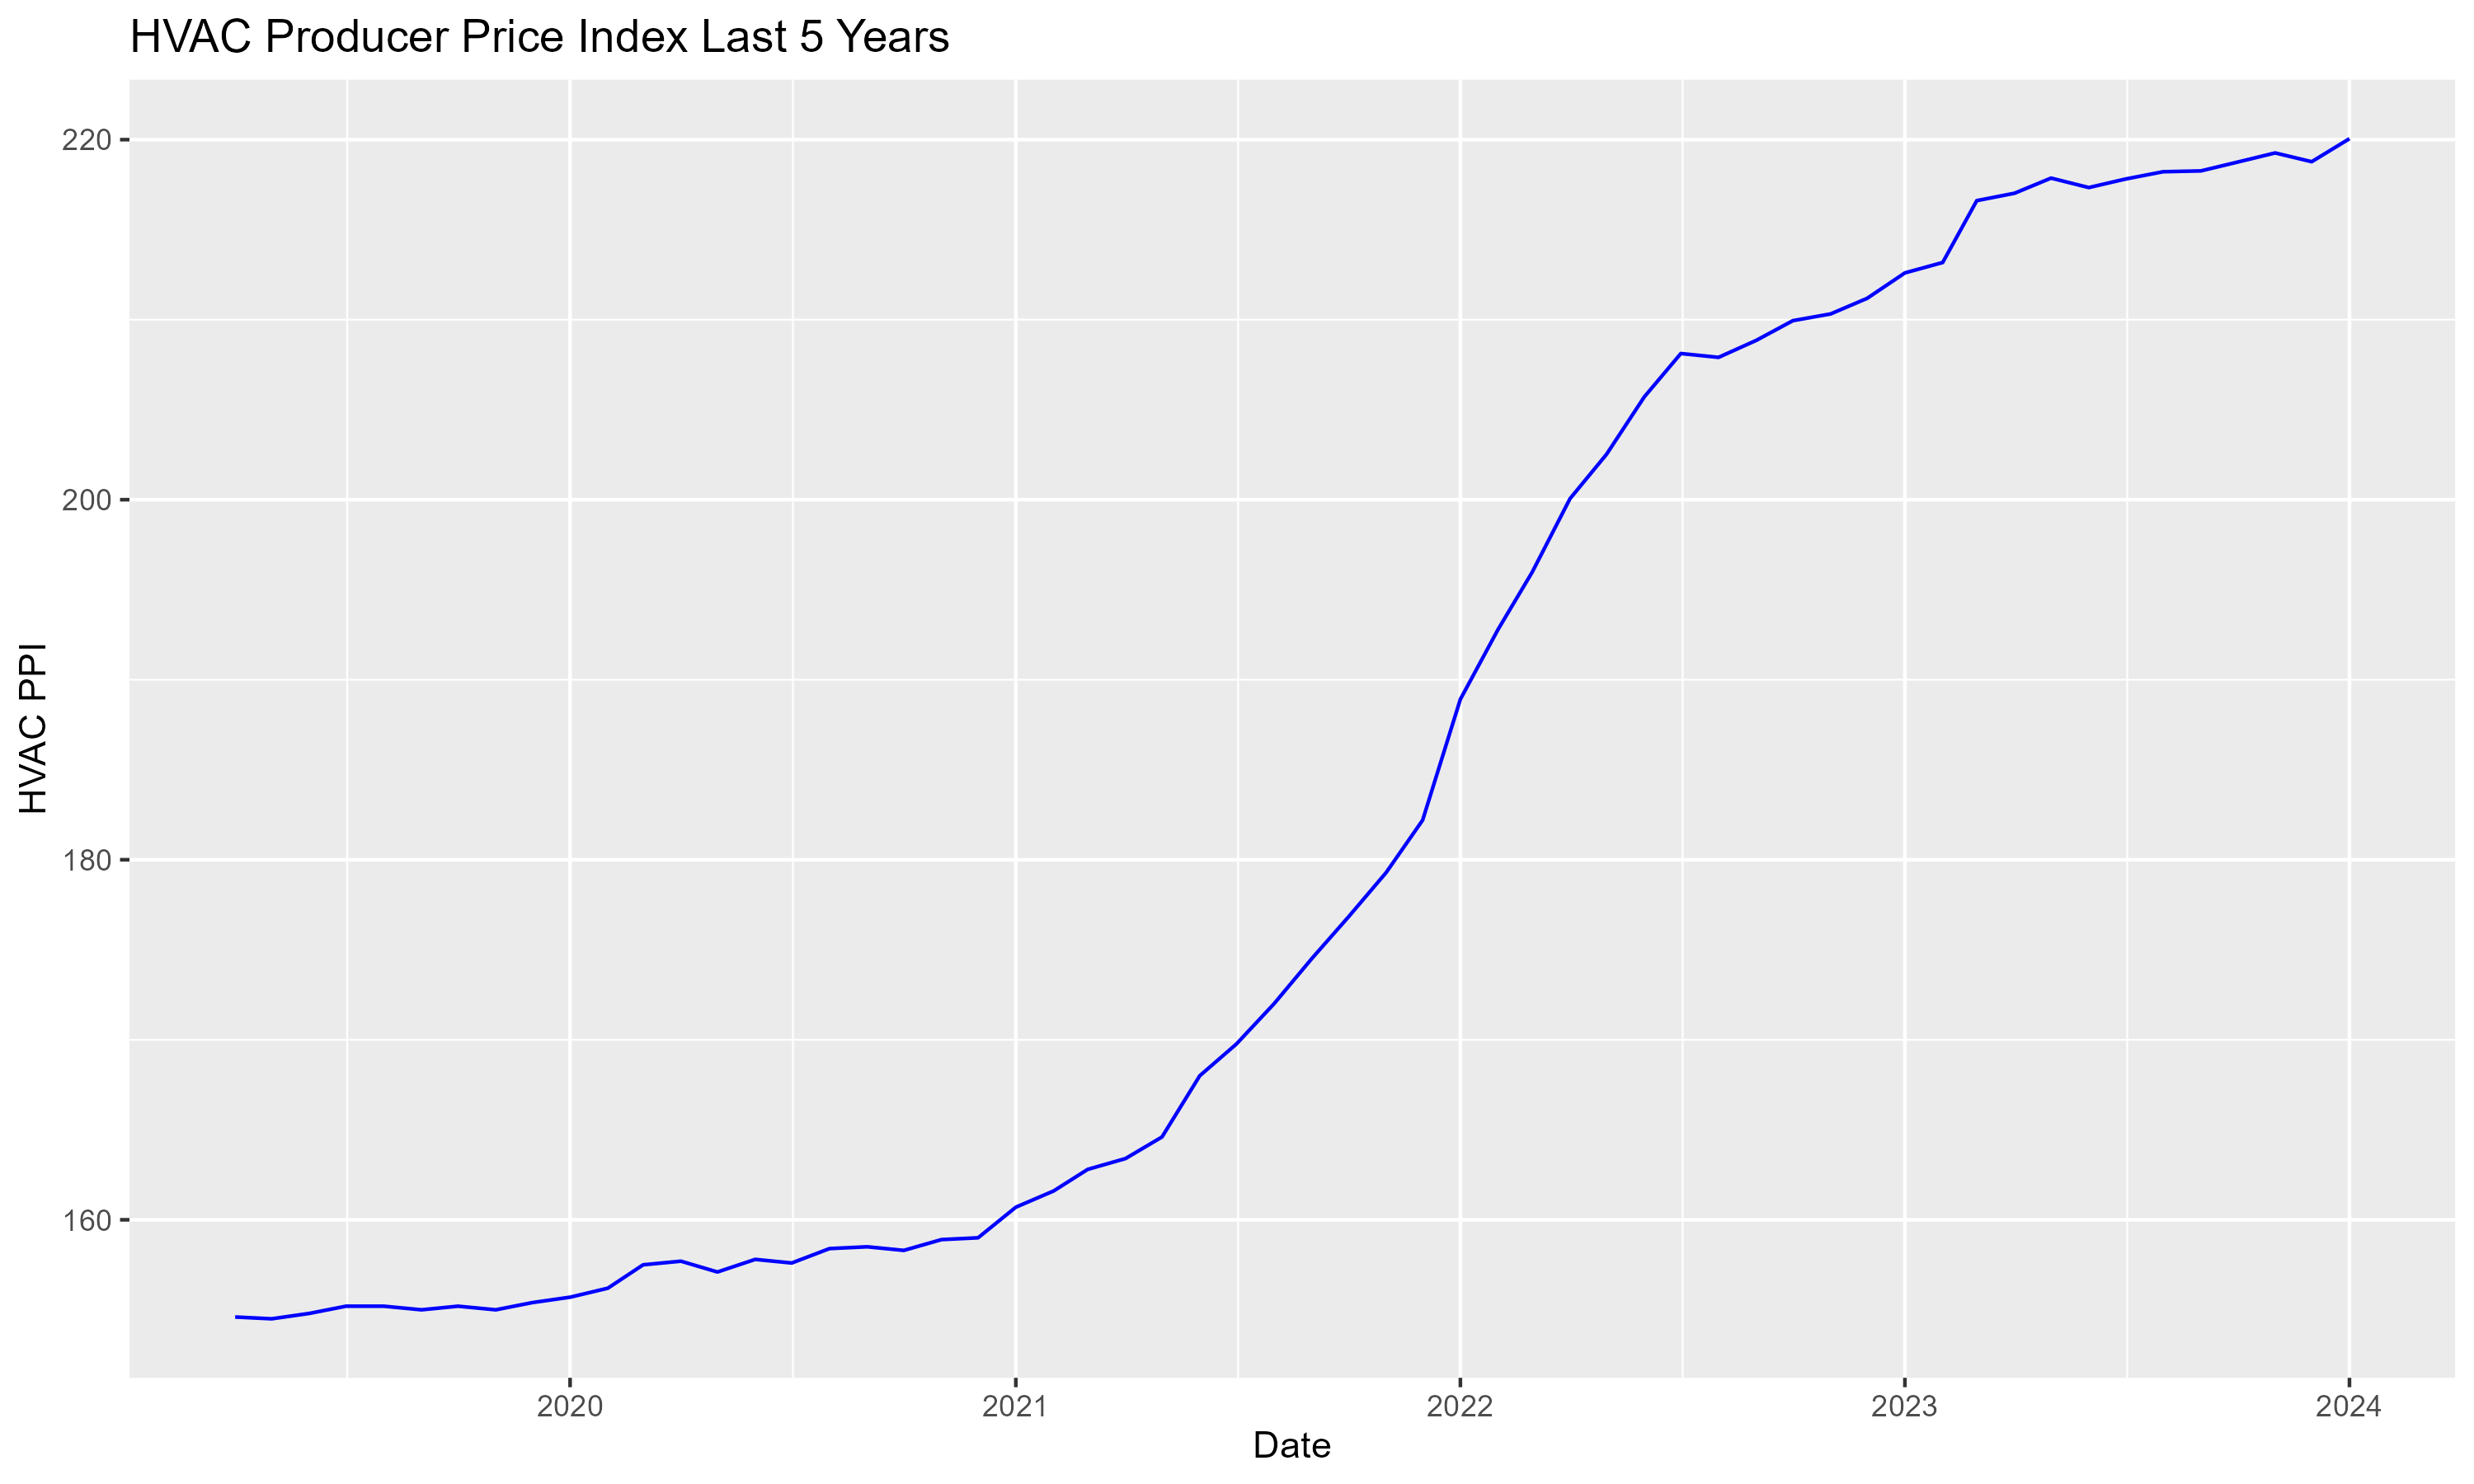
\includegraphics[width=1\linewidth]{PS6a_Smith.png}
        \caption{Time Series Plot of HVAC PPI}
        \label{fig:enter-label}
    \end{figure}
\end{enumerate}

\section{Question 4 Plot B}
\begin{enumerate}
\item The second Time series, Figure 2, plot displays the Percentage Change in HVAC PPI over the last 5 years, with respect to the older date. Although at first glance the line might look the same, it's another way to view the percentage increase from Q2 2019. Over a 40 percent increase is astounding, and it still does not appear to have leveled off or corrected down at all.
    \begin{figure}
        \centering
        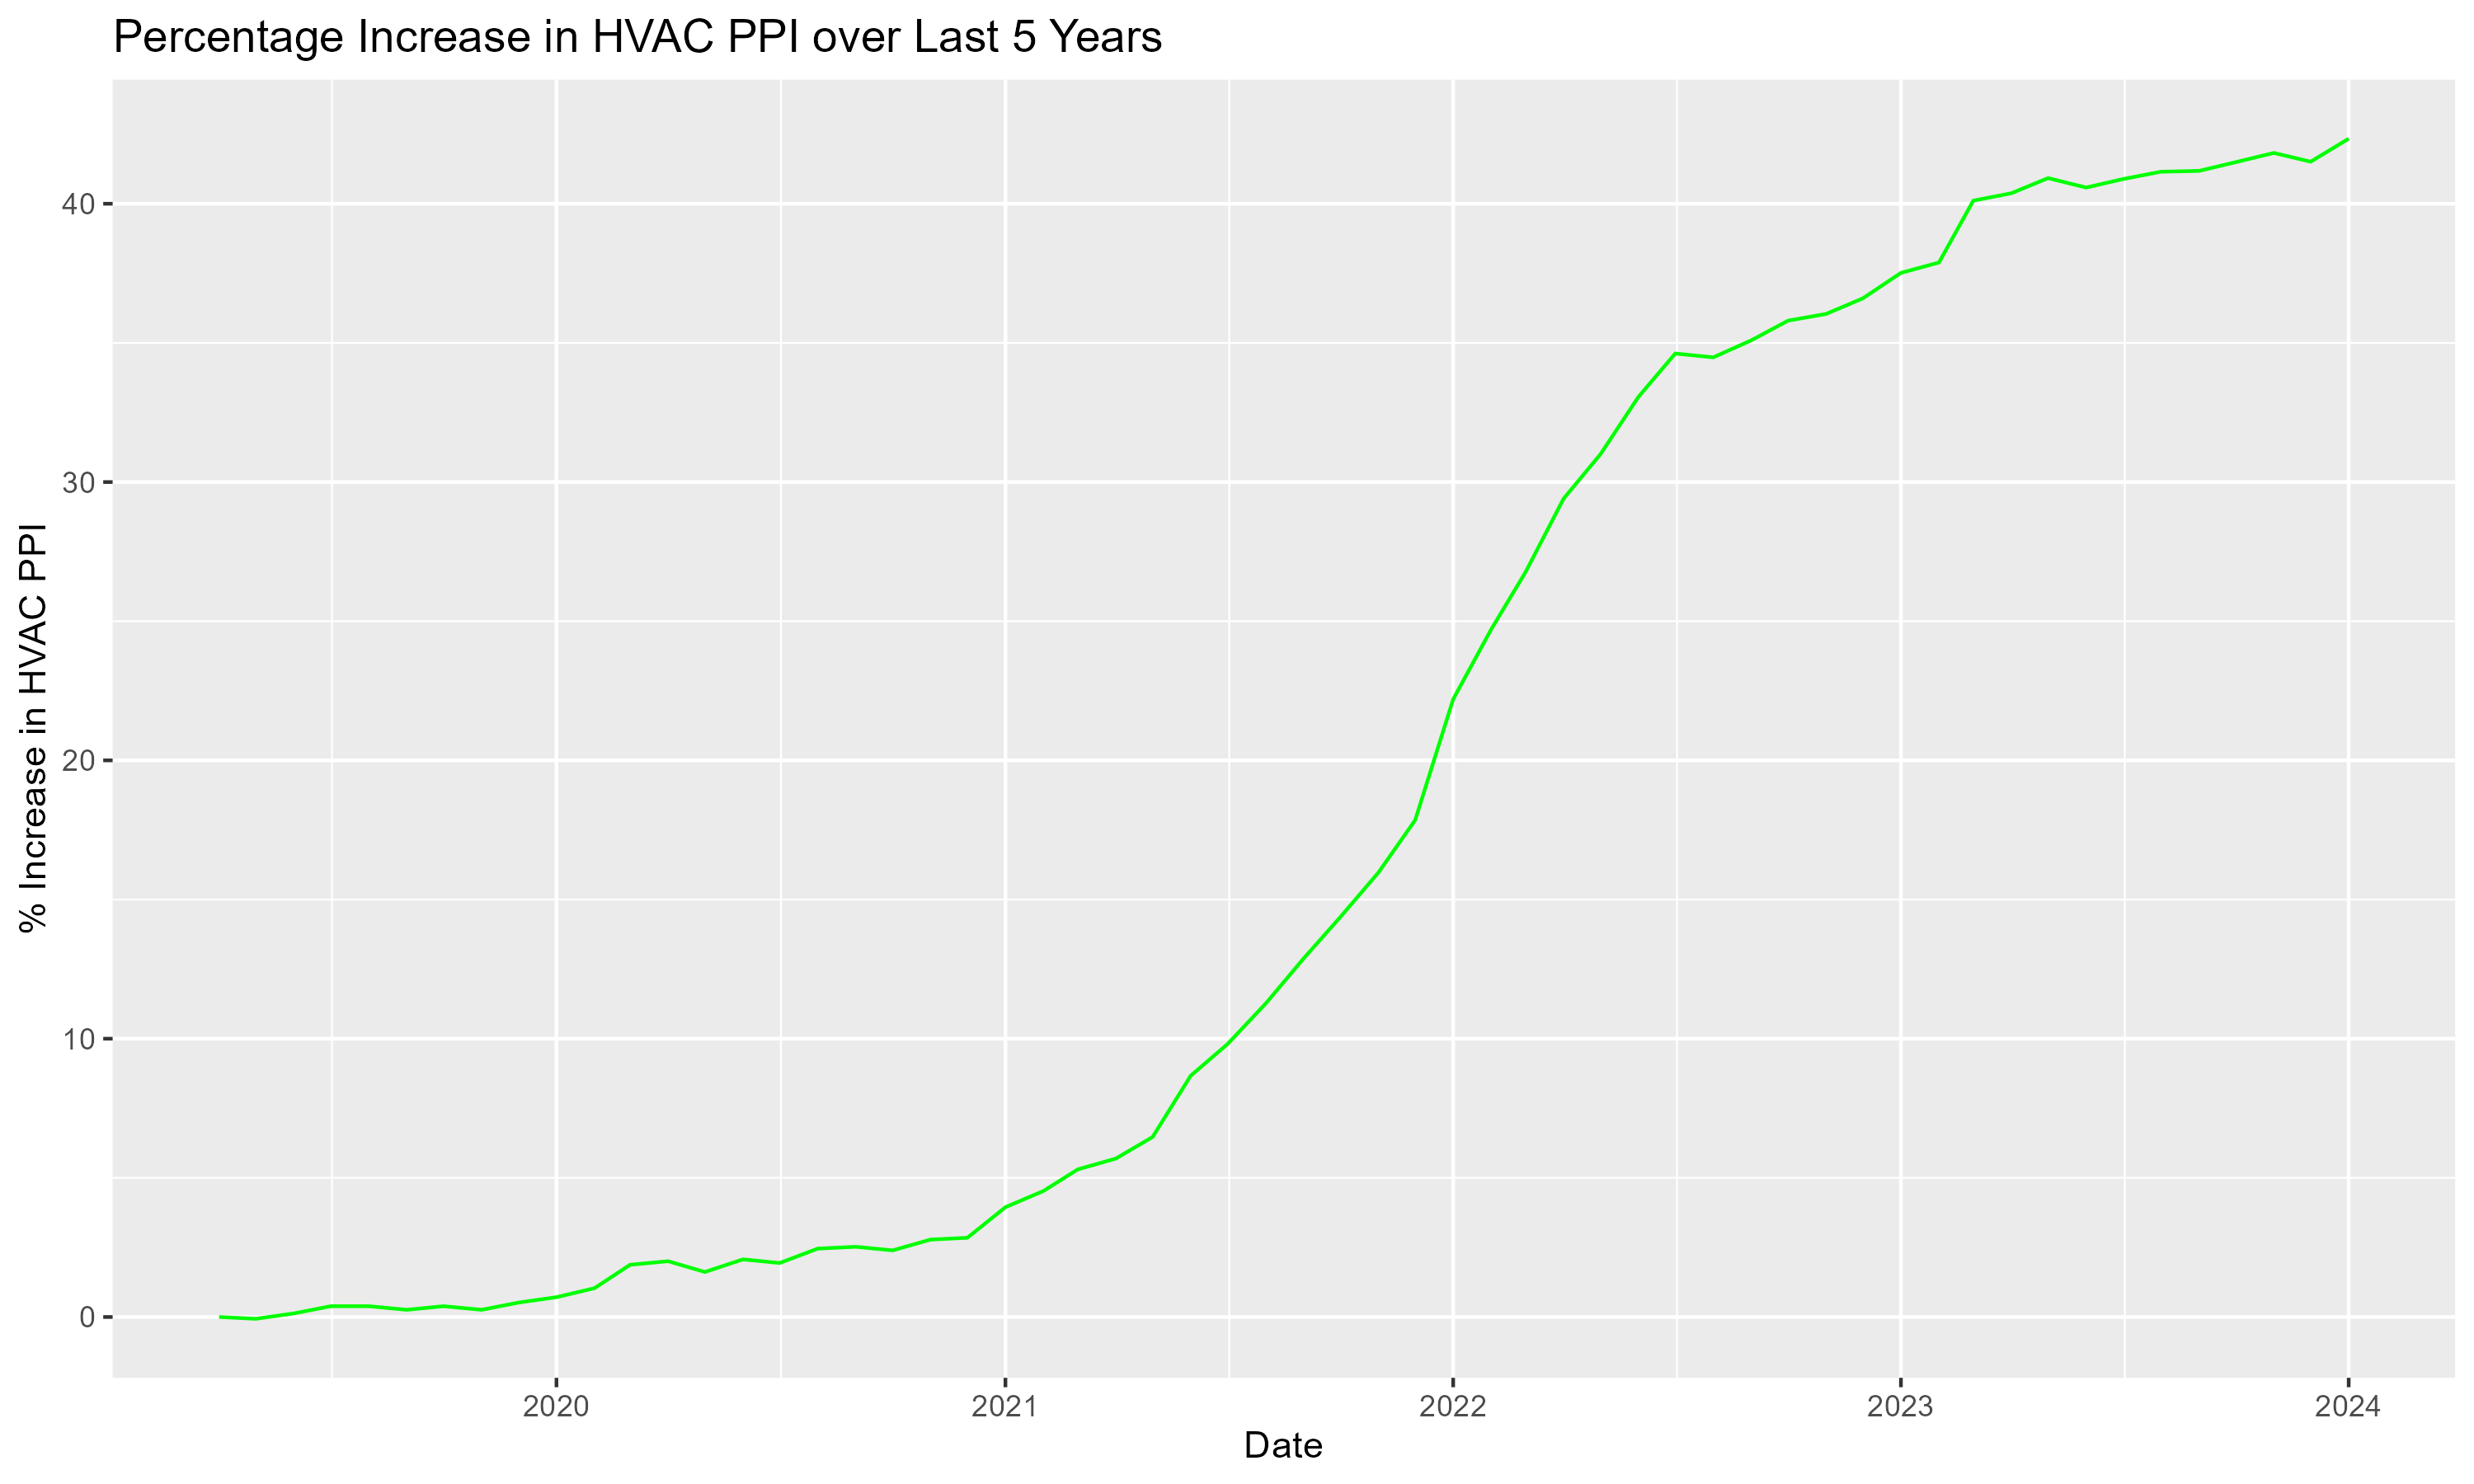
\includegraphics[width=1\linewidth]{PS6b_Smith.png}
        \caption{Time Series Percentage Increase Plot of HVAC PPI}
        \label{fig:enter-label}
    \end{figure}
\end{enumerate}

\section{Question 4 Plot C}
\begin{enumerate}
\item This last view, Figure 3, I had to create a secondary data frame to consolidate the dates by year and quarter. I also added a percentage change column, comparing quarter - to - quarter. This chart highlights the quarters that had the biggest increase in PPI compared to the previous time period. This shows a different way to view the rapid rate of increase that started in Q1 2021 through Q2 2022. Although all the values are still positive, the rate of change has been on the decline since Q1 2022.
    \begin{figure}
        \centering
        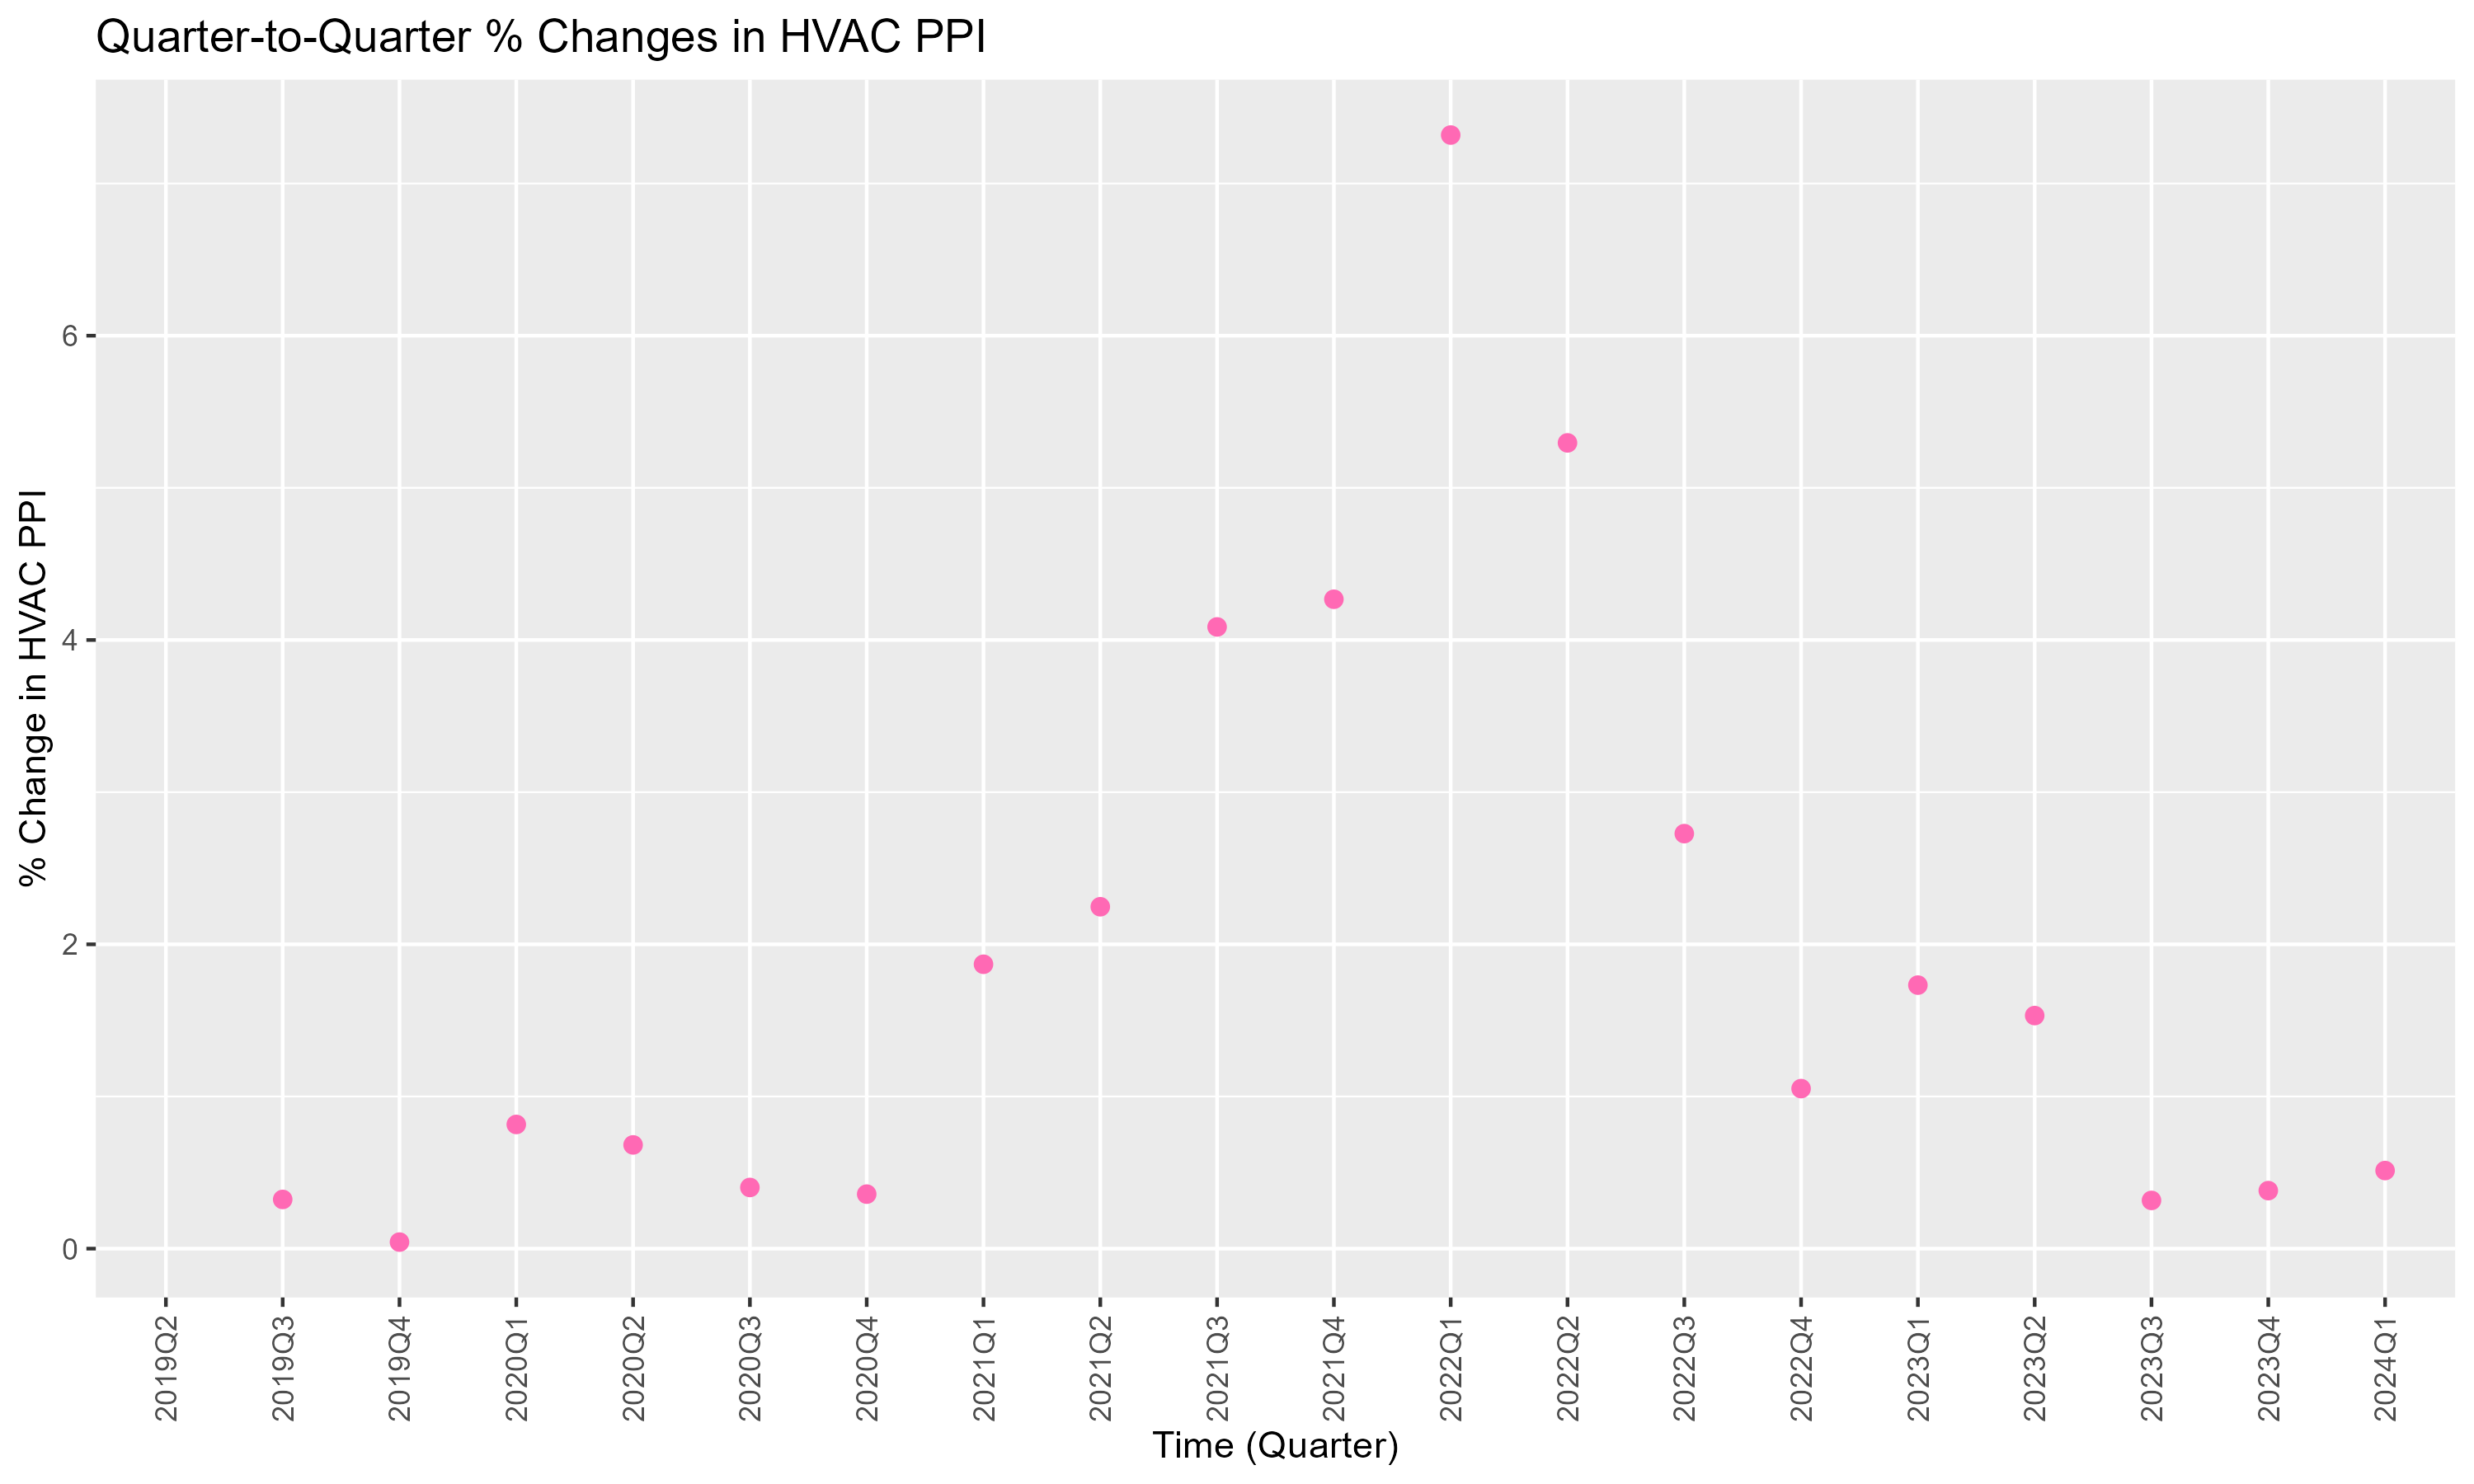
\includegraphics[width=1\linewidth]{PS6c_Smith.png}
        \caption{Quarter-to-Quarter Percentage Change in HVAC PPI}
        \label{fig:enter-label}
    \end{figure}
\end{enumerate}

\end{document}